% Preamble
\documentclass{beamer}
\usepackage[spanish]{babel}

% Packages
\usepackage{amsmath}
\usepackage[utf8]{inputenc}
\usepackage[T1]{fontenc}
\usepackage{graphicx}
\usepackage{algorithmicx}
\usepackage{algpseudocode}
\usepackage{caption}
\usepackage{courier}

\DeclareMathOperator{\atantwo}{atan2}

\captionsetup{justification=centering, font={scriptsize}, skip=0pt}

% Set bold vectors to satisfy requirements
\renewcommand\vec[1]{\ifstrequal{#1}{0}{\ensuremath{\mathbf{0}}}{\ensuremath{\boldsymbol{#1}}}}

\usetheme[compress]{Berlin}
\usecolortheme{wolverine}
\setbeamertemplate{page number in head/foot}[framenumber]
\setbeamercolor{institute in head/foot}{parent=palette primary}

\title[Dinámica peatonal]{Dinámica peatonal}
\subtitle{72.25 - Simulación de Sistemas}
\author[Flores Lucey, Llanos]{Alejo Flores Lucey\inst{1} \and Nehuén Gabriel Llanos\inst{2}}
\institute[Instituto Tecnológico de Buenos Aires]
{
    \inst{1}
    \href{mailto:afloreslucey@itba.edu.ar}{afloreslucey@itba.edu.ar}\\
    Legajo 62622
    \and
    \inst{2}
    \href{mailto:nllanos@itba.edu.ar}{nllanos@itba.edu.ar}\\
    Legajo 62511
}
\date{2024 1C | Grupo Nº3}
\titlegraphic{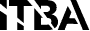
\includegraphics[height=0.5cm]{./itba}}

\makeatletter
\beamer@theme@subsectionfalse
\makeatother

\AtBeginSection[]{
    \begin{frame}
        \begin{beamercolorbox}[sep=8pt,center]{title}
            \usebeamerfont{title}\insertsection
        \end{beamercolorbox}
    \end{frame}
}

\begin{document}

    \begin{frame}
        \titlepage
    \end{frame}

    \section{Introducción}

        \begin{frame}{Introducción}
            \begin{itemize}
                \item Dinámica de interacción entre personas en movimiento.
                \item Simulación de un jugador virtual que sigue a la pelota durante un partido de fútbol en dos dimensiones.
            \end{itemize}
            \begin{minipage}[t]{0.5\textwidth}
                \begin{itemize}
                    \item Sistema real:
                    \begin{itemize}
                        \item Procesos de evacuación.
                        \item Predicción del flujo de personas.
                    \end{itemize}
                \end{itemize}
            \end{minipage}
            \hfill
            \begin{minipage}[t]{0.45\textwidth}
                \begin{figure}[H]
                    \centering
                    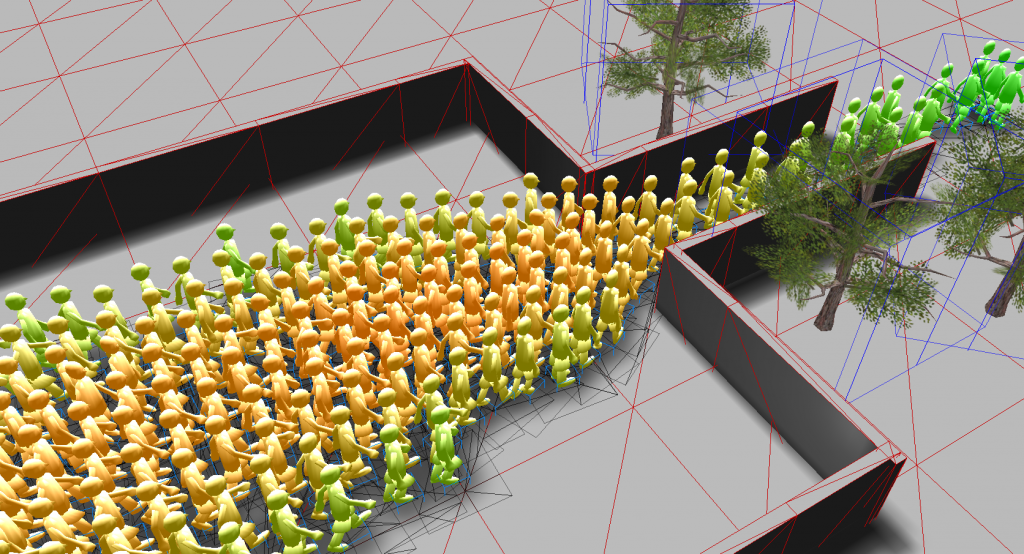
\includegraphics[width=\linewidth]{./sistema_real}
                    \label{fig:sistema_real}
                \end{figure}
            \end{minipage}
        \end{frame}

        \subsection{Fundamentos}

            \begin{frame}{Fundamentos: Social Force Model}
                \begin{itemize}
                    \item Sean $N$ peatones en un espacio bidimensional:
                        \begin{equation*}
                            m_i \cdot \vec{a}_i = \vec{F}_{i}^{(granular)} + \vec{F}_{i}^{(social)} + \vec{F}_{i}^{(deseo)}
                        \end{equation*}
                    \item Distancia entre peatones:
                        \begin{equation*}
                            \varepsilon_{ij} = d_{ij} - (R_i + R_j)
                        \end{equation*}
                    \item Fuerza granular:
                        \begin{equation*}
                            \vec{F}_{i}^{(granular)} = \sum_{j \neq i}^{N} -k_n \cdot g(\varepsilon_{ij}) \cdot \vec{e}_{ij}^{n}\ ;\ g(w) = \begin{cases} w & \text{si } w < 0 \\ 0 & \text{si } w \geq 0 \end{cases}
                        \end{equation*}
                \end{itemize}
                \begin{minipage}[t]{0.49\textwidth}
                    \begin{itemize}
                        \item Fuerza social:
                        \begin{equation*}
                            \vec{F}_{i}^{(social)} = \sum_{j \neq i}^{N} A \cdot e^{\frac{-\varepsilon_{ij}}{B}} \cdot \vec{e}_{ij}^{n}
                        \end{equation*}
                    \end{itemize}
                \end{minipage}
                \hfill
                \begin{minipage}[t]{0.49\textwidth}
                    \begin{itemize}
                        \item Fuerza de deseo:
                        \begin{equation*}
                            \vec{F}_{i}^{(deseo)} = m_i \cdot \frac{\vec{v}_i^{deseo} - \vec{v}_i}{\tau}
                        \end{equation*}
                    \end{itemize}
                \end{minipage}
            \end{frame}

    \section{Implementación}

        \subsection{Arquitectura}

            \begin{frame}{Diagrama UML}
                \begin{figure}[htbp]
                    \centering
                    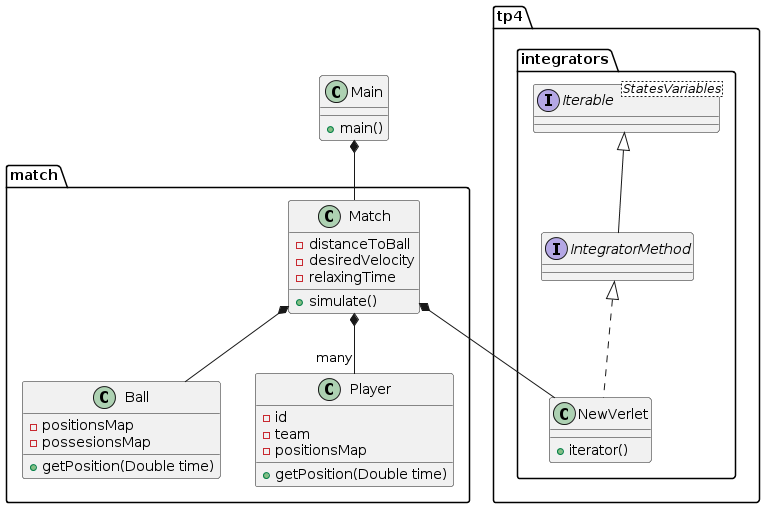
\includegraphics[width=\textwidth]{./architecture}
                    \label{fig:architecture}
                \end{figure}
            \end{frame}

        \subsection{Algoritmo}

            \begin{frame}{Pseudocódigo del algoritmo implementado}{}
                \begin{algorithmic}[1]
                    \ttfamily \scriptsize
                    \State Create output file
                    \State accX $\gets$ \Call{function}{ball, players}
                    \State accY $\gets$ \Call{function}{ball, players}
                    \State integrators $\gets$ [accX, accY]
                    \State $t$ $\gets$ startTime
                    \State $i$ $\gets$ 0
                    \While{$t$ $<$ endTime}
                        \State crazyGuyX, crazyGuyY $\gets$ \Call{integrators.next}{}()
                        \State \Call{UpdateStateVariables}{crazyGuyX, crazyGuyY}
                        \If{$i \equiv 0(10)$}
                            \State \Call{WriteOutput}{crazyGuyX, crazyGuyY}
                        \EndIf
                        \State $t \gets t + dt$
                        \State $i \gets i + 1$
                    \EndWhile
                \end{algorithmic}
            \end{frame}

    \section{Simulaciones}

        \subsection{Parámetros de entrada}

            \begin{frame}{Parámetros de entrada}
                \begin{itemize}
                    \item Parámetros de entrada fijos:
                    \begin{itemize}
                        \item $d_{pelota-loco}$: \alert{$10$ m}
                        \item $R_{jugadores}$: \alert{$0.3$ m}
                        \item $m_{jugadores}$: \alert{$80$ kg}
                        \item $r_{jugador_i}$: \alert{[$(x, y)$, ...]}
                    \end{itemize}
                    \item Parámetros de entrada variables:
                    \begin{itemize}
                        \item $v_d$: \alert{${0.1; 1; 2; 3; 4; ...; 13}$ m/s}
                        \item $\tau$: \alert{$0.1; 0.2; ...; 1$ s}
                    \end{itemize}
                \end{itemize}
                \begin{block}{Dato curioso}
                    Como método de integración se utilizó \textbf{Verlet 2.0}, presentado en el TP anterior.
                \end{block}
            \end{frame}

        \subsection{Cálculo de variables importantes}

            \begin{frame}{Elección del periodo de simulación}
                \begin{itemize}
                    \item Se busca un periodo \alert{$[t_i ; t_f]$} tal que:
                    \begin{itemize}
                        \item $t_i > 120$ s $\land\ t_f < 6000$ s
                        \item Se mantengan los mismos jugadores en la cancha.
                        \item $x_{pelota} \ne$ NaN $\land\ y_{pelota} \ne$ NaN $\forall t \in [t_i ; t_f]$
                    \end{itemize}
                    \item Se encuentra que:
                    \begin{itemize}
                        \item $\max\{[t_i ; t_f] : \text{mismos jugadores en la cancha}\} = [0.04 ; 3519.40]$
                        \item $\max\{[t_i ; t_f] : x_{pelota} \ne \text{NaN} \land\ y_{pelota} \ne \text{NaN}\} = [57.24 ; 177.72]$
                    \end{itemize}
                \end{itemize}
                \begin{beamercolorbox}[sep=5pt,center]{block body}
                    \centering
                    $\therefore [t_i ; t_f] = [57.24 ; 177.72] \Rightarrow D = 120.48$ s
                \end{beamercolorbox}
            \end{frame}

            \begin{frame}{Cálculo de la velocidad de deseo en cada instante}
                \begin{itemize}
                    \item Tomamos el módulo de la velocidad de deseo de parámetro de entrada.
                    \item Obtenemos la velocidad de deseo en cada instante $t$:
                        \begin{equation*}
                            \hat{e_n} = \frac{\vec{r}(t)_{pelota} - \vec{r}(t)_{loco}}{||\vec{r}(t)_{pelota} - \vec{r}(t)_{loco}||}= (e_n \hat{\imath}, e_n \hat{\jmath})
                        \end{equation*}
                        \begin{equation*}
                            \vec{v_d} = |v_d| \cdot \hat{e_n}
                        \end{equation*}
                \end{itemize}
            \end{frame}

        \subsection{Observables}

            \begin{frame}{Distancia entre el jugador virtual y la pelota}
                \begin{equation*}
                    d = \sqrt{(x_{pelota} - x_{loco})^2 + (y_{pelota} - y_{loco})^2} - R_{loco}
                \end{equation*}
                \begin{itemize}
                    \item Se busca minimizar la distancia entre el jugador virtual y la pelota, variando $v_d$ y $\tau$.
                    \item $d$ no presenta un comportamiento gaussiano $\Rightarrow$ Cuando se toman promedios, el error se calcula como:
                    \begin{equation*}
                        E = \frac{\sigma}{\sqrt{N}}\ ;\ \sigma = \text{desvío estándar}\ ;\ N = \text{cantidad de datos}
                    \end{equation*}
                \end{itemize}
            \end{frame}

            \begin{frame}{Módulo de la velocidad de distintos jugadores}
                \begin{equation*}
                    \vec{v}(t) = \frac{\vec{r}(t) - \vec{r}(t - \Delta t)}{\Delta t}\ ;\ \Delta t = 0.04 \text{s}
                \end{equation*}
                \begin{itemize}
                    \item Se eliminan las velocidades que superen los $TODO$ m/s.
                    \item Se estudia la función de densidad de probabilidad de la velocidad de los jugadores.
                    \begin{itemize}
                        \item Se calcula el número de bins usando la \alert{regla de Sturges}.
                        \item Se calcula el ancho de los bins usando el \alert{método de Scott}.
                    \end{itemize}
                \end{itemize}
            \end{frame}

            \begin{frame}{Número de visitas a zonas de la cancha por minuto ($\Psi$)}
                \begin{itemize}
                    \item Se divide la cancha en zonas de $TODO \times TODO \text{ m}^2$.
                    \begin{equation*}
                        \Psi = \frac{\sum_{i \in \text{jugadores}} \#visitas_i}{D}
                    \end{equation*}
                    \begin{equation*}
                        D = \text{periodo de simulación} = 2.008 \text{ minutos}
                    \end{equation*}
                    \item Se estudia $\Psi$ utilizando un \alert{heatmap}.
                \end{itemize}
            \end{frame}

    \section{Resultados}

        \subsection{Animación del sistema}

            \begin{frame}{Animación del sistema}{}
                \vspace*{-0.3cm}
                \begin{figure}[H!]
                    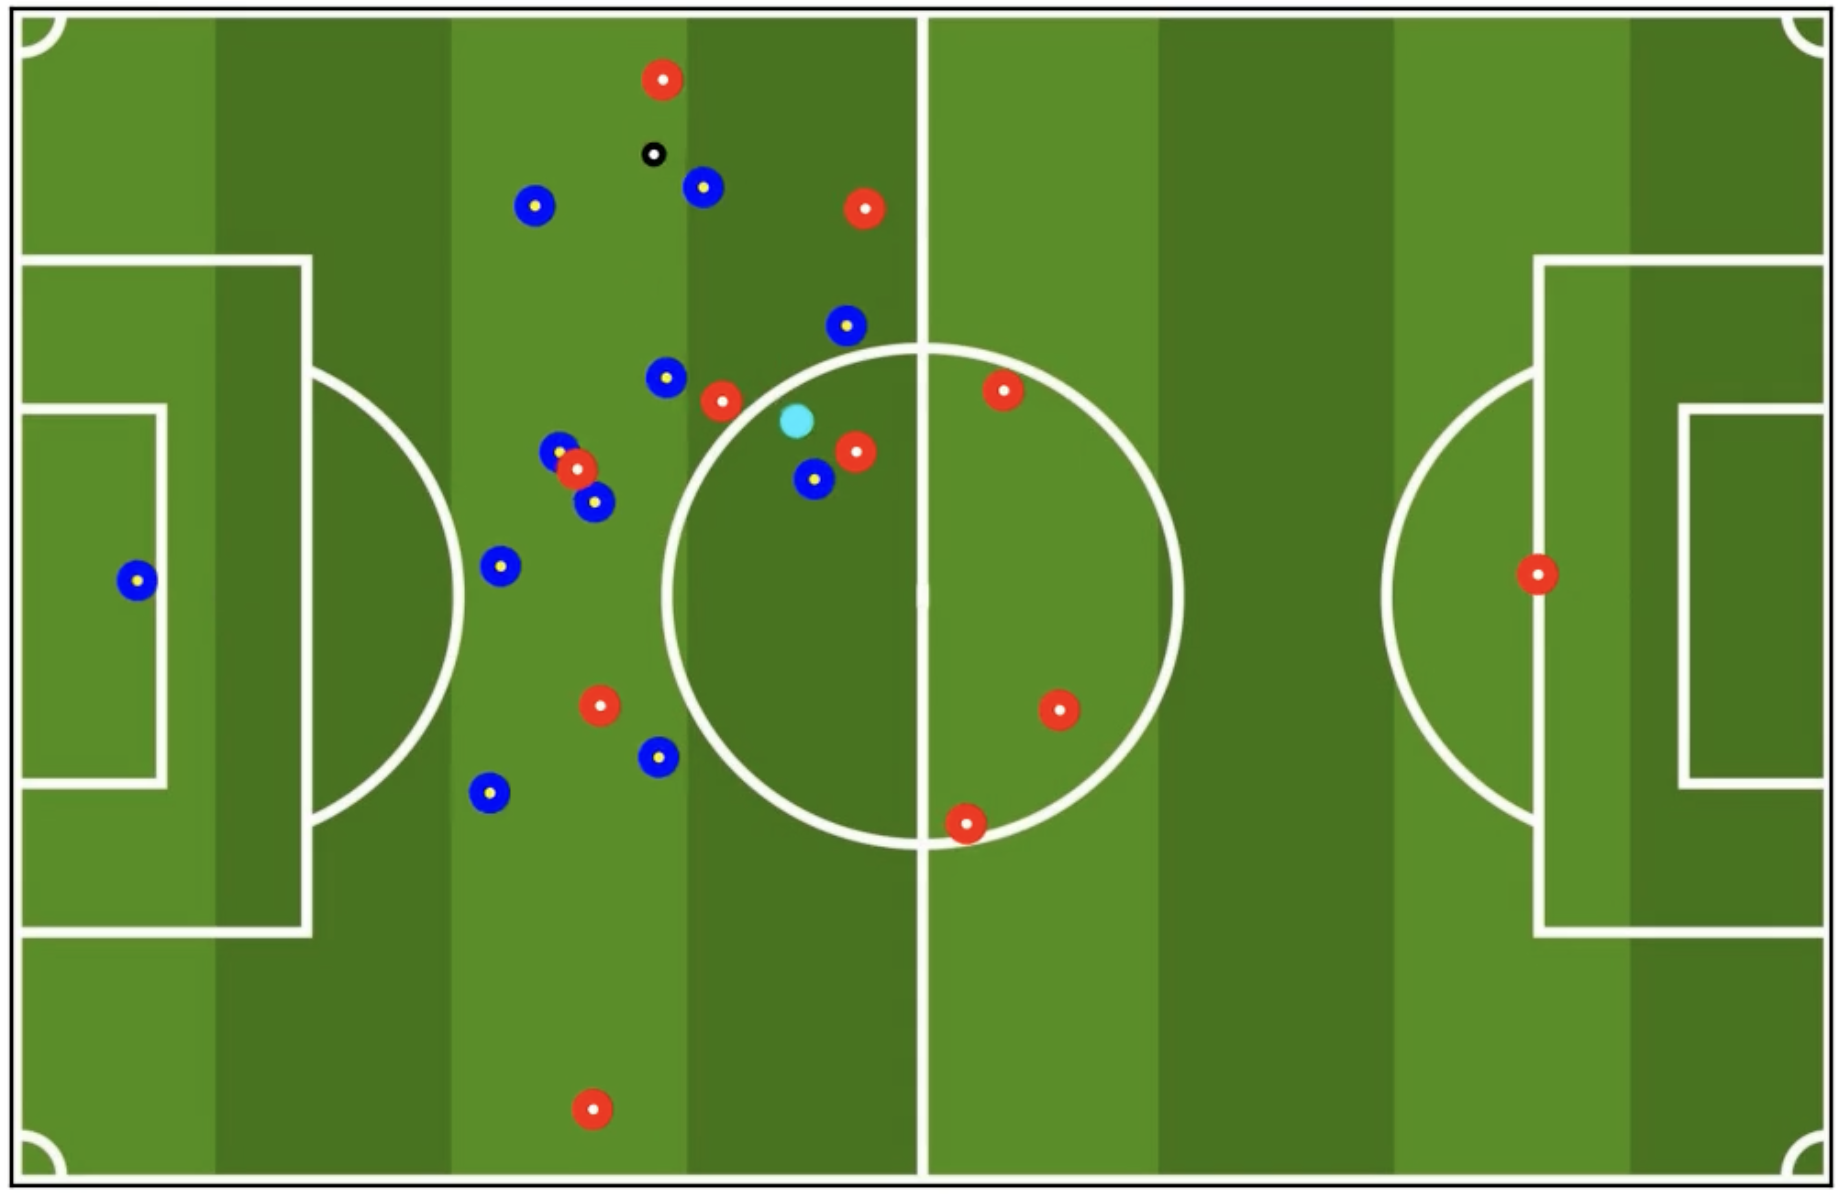
\includegraphics[width=\textwidth]{./animacion_1}
                    \caption*{Véase la animación completa en \url{TODO}.}
                    \label{fig:futbol_1}
                \end{figure}
                \vspace*{-0.5cm}
                \begin{beamercolorbox}[sep=5pt,center]{block body}
                    \centering
                    \small{$v_d = 5$ m/s ; $\tau = 0.5$ s}
                \end{beamercolorbox}
            \end{frame}

        \subsection{Elección del $\Delta t$}

            \begin{frame}{Energía perdida en función del tiempo}{Elección del $\Delta t$}
                    \begin{figure}[H!]
                        \includegraphics[width=0.9\textwidth]{./energia_perdida_vs_tiempo}
                        \label{fig:marte_3}
                    \end{figure}
                    \begin{beamercolorbox}[sep=5pt,center]{block body}
                        \centering
                        \small{Estudio en 50 días}
                    \end{beamercolorbox}
            \end{frame}

            \begin{frame}{Promedio de energía perdida vs $\Delta t$}{Elección del $\Delta t$}
                \begin{figure}[H!]
                    \includegraphics[width=0.9\textwidth]{./promedio_energia_perdida_vs_dt}
                    \label{fig:marte_4}
                \end{figure}
                \begin{beamercolorbox}[sep=5pt,center]{block body}
                    \centering
                    \small{Estudio en 50 días}
                \end{beamercolorbox}
            \end{frame}

        \subsection{Momento óptimo de partida para arribar a Marte}

            \begin{frame}{Distancia mínima a Marte vs día de partida}{Momento óptimo de partida para arribar a Marte}
                \begin{figure}[H!]
                    \includegraphics[width=0.9\textwidth]{./distancia_a_marte_vs_dia_de_partida}
                    \label{fig:marte_5}
                \end{figure}
                \begin{beamercolorbox}[sep=5pt,center]{block body}
                    \centering
                    \small{$\Delta t = 60s$ ; Misión exitosa si $d_{nave-marte} < 3520 km$}
                \end{beamercolorbox}
            \end{frame}

            \begin{frame}{Distancia mínima a Marte vs hora de partida}{Momento óptimo de partida para arribar a Marte. A partir de 171d}
                \begin{figure}[H!]
                    \includegraphics[width=0.9\textwidth]{./distancia_a_marte_vs_hora_de_partida}
                    \label{fig:marte_6}
                \end{figure}
                \begin{beamercolorbox}[sep=5pt,center]{block body}
                    \centering
                    \small{$\Delta t = 60s$ ; Misión exitosa si $d_{nave-marte} < 3520 km$}
                \end{beamercolorbox}
            \end{frame}

            \begin{frame}{Distancia mínima a Marte vs minuto de partida}{Momento óptimo de partida para arribar a Marte. A partir de 171d 22h}
                \begin{figure}[H!]
                    \includegraphics[width=0.9\textwidth]{./distancia_a_marte_vs_minuto_de_partida}
                    \label{fig:marte_7}
                \end{figure}
                \begin{beamercolorbox}[sep=5pt,center]{block body}
                    \centering
                    \small{$\Delta t = 60s$ ; $d_{nave-marte} = 2547.98 km$}
                \end{beamercolorbox}
            \end{frame}

        \subsection{Velocidad de la nave vs tiempo}

            \begin{frame}{Módulo de la velocidad de la nave vs tiempo}{Partida de la nave: 171d 23h 17m}
                \begin{figure}[H!]
                    \includegraphics[width=0.9\textwidth]{./velocity_vs_time_for_travel_to_mars}
                    \label{fig:marte_8}
                \end{figure}
                \begin{beamercolorbox}[sep=5pt,center]{block body}
                    \centering
                    \small{$\Delta t = 60s$ ; $t_{vuelo} = 81d 15h 5m$}
                \end{beamercolorbox}
            \end{frame}

        \subsection{Variación de la velocidad incial de la nave}

            \begin{frame}{Distancia mínima a Marte vs velocidad inicial de la nave}{Partida de la nave: 171d 23h 17m}
                \begin{figure}[H!]
                    \includegraphics[width=0.9\textwidth]{./min_distance_vs_v0_logaritmica_line_in_10^4_scatter}
                    \label{fig:marte_9}
                \end{figure}
                \begin{beamercolorbox}[sep=5pt,center]{block body}
                    \centering
                    \small{$\Delta t = 60s$ ; Misión exitosa si $d_{nave-marte} < 10^4 km$}
                \end{beamercolorbox}
            \end{frame}

            \begin{frame}{Distancia mínima a Marte vs velocidad inicial de la nave}{Partida de la nave: 171d 23h 17m}
                \begin{figure}[H!]
                    \includegraphics[width=0.9\textwidth]{./min_distance_vs_v0_logaritmica_line_in_10^4_reduced_scatter}
                    \label{fig:marte_10}
                \end{figure}
                \begin{beamercolorbox}[sep=5pt,center]{block body}
                    \centering
                    \small{$\Delta t = 60s$ ; Misión exitosa si $d_{nave-marte} < 10^4 km$}
                \end{beamercolorbox}
            \end{frame}

            \begin{frame}{Tiempo de vuelo vs velocidad inicial de la nave}{Partida de la nave: 171d 23h 17m}
                \begin{figure}[H!]
                    \includegraphics[width=0.9\textwidth]{./time_vs_v0_for_v_less_10^4_scatter}
                    \label{fig:marte_11}
                \end{figure}
                \begin{beamercolorbox}[sep=5pt,center]{block body}
                    \centering
                    \small{$\Delta t = 60s$ ; Misión exitosa si $d_{nave-marte} < 10^4 km$}
                \end{beamercolorbox}
            \end{frame}

        \subsection{Sistema con Júpiter}

            \begin{frame}{Animación del sistema}{}
                \vspace*{-0.3cm}
                \begin{minipage}[t]{0.49\textwidth}
                    \begin{figure}[H!]
                        \includegraphics[width=\textwidth]{./animacion_jupiter_1}
                        \caption*{Véase la animación completa en \url{https://youtu.be/uGcs41rDAmk}.}
                        \label{fig:jupiter_1}
                    \end{figure}
                    \vspace*{-0.5cm}
                    \begin{beamercolorbox}[sep=5pt,center]{block body}
                        \centering
                        \small{Día de partida: 0}
                    \end{beamercolorbox}
                \end{minipage}
                \hfill
                \begin{minipage}[t]{0.49\textwidth}
                    \begin{figure}[H!]
                        \includegraphics[width=\textwidth]{./animacion_jupiter_2}
                        \caption*{Véase la animación completa en \url{https://youtu.be/GijCuivfah8}.}
                        \label{fig:jupiter_2}
                    \end{figure}
                    \vspace*{-0.5cm}
                    \begin{beamercolorbox}[sep=5pt,center]{block body}
                        \centering
                        \small{Día de partida: 896}
                    \end{beamercolorbox}
                \end{minipage}
            \end{frame}

            \begin{frame}{Distancia mínima a Júpiter vs día de partida}{Momento óptimo de partida para arribar a Júpiter}
                \begin{figure}[H!]
                    \includegraphics[width=0.9\textwidth]{./distancia_a_jupiter_vs_dia_de_partida}
                    \label{fig:jupiter_3}
                \end{figure}
                \begin{beamercolorbox}[sep=5pt,center]{block body}
                    \centering
                    \small{$\Delta t = 60s$ ; Misión exitosa si $d_{nave-jupiter} < 71000 km$}
                \end{beamercolorbox}
            \end{frame}

            \begin{frame}{Distancia mínima a Júpiter vs hora de partida}{Momento óptimo de partida para arribar a Júpiter. A partir de 895d}
                \begin{figure}[H!]
                    \includegraphics[width=0.9\textwidth]{./distancia_a_jupiter_vs_hora_de_partida}
                    \label{fig:jupiter_4}
                \end{figure}
                \begin{beamercolorbox}[sep=5pt,center]{block body}
                    \centering
                    \small{$\Delta t = 60s$ ; Misión exitosa si $d_{nave-jupiter} < 71000 km$}
                \end{beamercolorbox}
            \end{frame}

            \begin{frame}{Distancia mínima a Júpiter vs minuto de partida}{Momento óptimo de partida para arribar a Júpiter. A partir de 896d 1h}
                \begin{figure}[H!]
                    \includegraphics[width=0.9\textwidth]{./distancia_a_jupiter_vs_minuto_de_partida}
                    \label{fig:jupiter_5}
                \end{figure}
                \begin{beamercolorbox}[sep=5pt,center]{block body}
                    \centering
                    \small{$\Delta t = 60s$ ; $d_{nave-jupiter} = 705125 km$}
                \end{beamercolorbox}
            \end{frame}

            \begin{frame}{Distancia mínima a Júpiter vs velocidad inicial de la nave}{Partida de la nave: 896d 1h 52m}
                \begin{figure}[H!]
                    \includegraphics[width=0.9\textwidth]{./min_distance_vs_v0_logarithmic_jupiter}
                    \label{fig:jupiter_6}
                \end{figure}
                \begin{beamercolorbox}[sep=5pt,center]{block body}
                    \centering
                    \small{$\Delta t = 60s$ ; Misión exitosa si $d_{nave-jupiter} < 10^6 km$}
                \end{beamercolorbox}
            \end{frame}

            \begin{frame}{Tiempo de vuelo vs velocidad inicial de la nave}{Partida de la nave: 896d 1h 52m}
                \begin{figure}[H!]
                    \includegraphics[width=0.9\textwidth]{./travel_time_vs_v0_logarithmic_jupiter}
                    \label{fig:jupiter_7}
                \end{figure}
                \begin{beamercolorbox}[sep=5pt,center]{block body}
                    \centering
                    \small{$\Delta t = 60s$ ; Misión exitosa si $d_{nave-jupiter} < 10^6 km$}
                \end{beamercolorbox}
            \end{frame}

    \section{Conclusiones}

        \begin{frame}{Conclusiones}
            \begin{itemize}
                \item El óptimo $\Delta t$ tiene un mínimo.
                Llega un punto que si se sigue disminuyendo, el error es mayor.
                \item Los cambios en la velocidad inicial de la nave resultan en una mayor distancia mínima a Marte.
                \item A medida que la nave se aleja del sol, su aceleración disminuye.
                \item Estas observaciones se pueden extrapolar a otros sistemas planetarios.
            \end{itemize}
        \end{frame}

        \begin{frame}
            \begin{beamercolorbox}[sep=8pt,center]{title}
                \usebeamerfont{title}{¡Muchas gracias!}
            \end{beamercolorbox}
        \end{frame}

\end{document}
